\chapter {Test-driven development}

In the chapter about implementation, we mentioned that tests were written during implementation and that \acrshort{tdd}
technique was used. "Test-driven development is a software development approach in which test cases are developed to specify
and validate what the code will do." \cite{hamilton_what_2020} What this means to us, is that before the implementation of
our library, we should write a set of tests for our public \acrshort{api}. In this chapter we will focus on the implementation of the tests
and some base principles of test-driven development and testing in general.

To write tests we need a framework that will help us write these tests. In .NET there are number of test frameworks that we can use, here is a list of
the most used ones:

\begin{itemize}
    \item {MSTest - Microsoft original test framework}
    \item {NUnit - Originaly ported from JUnit \cite{noauthor_nunitorg_nodate}}
    \item {xUnit - Created by author of the NUnit v2 \cite{noauthor_home_nodate}}
\end{itemize}

Per author's experience, we will use the xUnit framework, but this type of testing is available in any of these frameworks.

.NET \acrshort{cli} tool has a template for xUnit project avaiable under command \texttt{dotnet new xunit}. Using this command will
prepare project with dependencies for xUnit and Microsoft.NET.Test.Sdk packages. It will also configure runners and coverlet.collector for collecting
code coverage.

\section{More information about \acrshort{tdd}}

Test-driven development can be summed using an activity diagram, at the start of the development, we write down all the tests that we need to cover our code
and then we start with implementation of library, at the end we factor our code, for example, we mode code from one method into multiple methods and even classes.
After refactoring is done, we then check our tests and write new ones.

\begin{figure}[H]
    \centering
    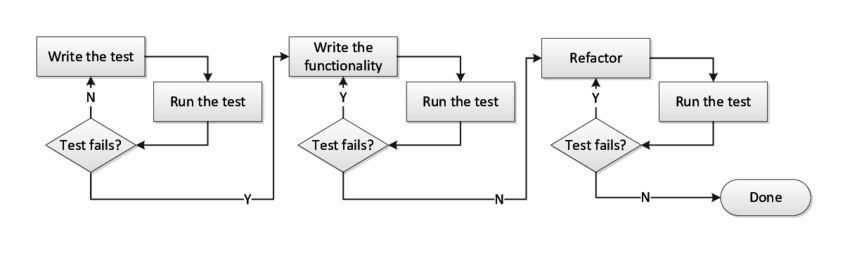
\includegraphics[width=\textwidth]{content/Test-Driven-Development-activities.png}
    \caption{Test-driven development diagram \cite{noauthor_continuous_2013}}
    \label{fig:tddDiagram}
\end{figure}

Using this approach has many benefits, one them is complete code coverage of our code, which means that every line should be covered by tests. To calculate
the coverage, we are going to use coverlet tool, which is cross platform coverage framework for .NET. \cite{noauthor_coverlet_2022} It supports multiple output
formats, but for our case, we will use \texttt{lcov} format, which can be then loaded by extension in Visual Studio Code and display coverage information directly in files.
We can also generate a report of the coverage using these commands.
\begin{itemize}
    \item {\texttt{dotnet test \textbackslash\\
              /p:CollectCoverage=true \textbackslash\\/p:CoverletOutput=../../lcov.info \textbackslash\\/p:CoverletOutputFormat=lcov}}
    \item {\texttt{genhtml lcov.info -o ./CoveragerReport/}}
\end{itemize}
First command is to execute test and generate \texttt{lcov.info} file, which contains coverage information, this file is also used by extension for Visual Studio Code
named Coverage Gutters.
Second command is to generate html report from \texttt{lcov.info} file.

Here \ref{fig:report} is an example of the report from this project.

\begin{figure}[H]
    \centering
    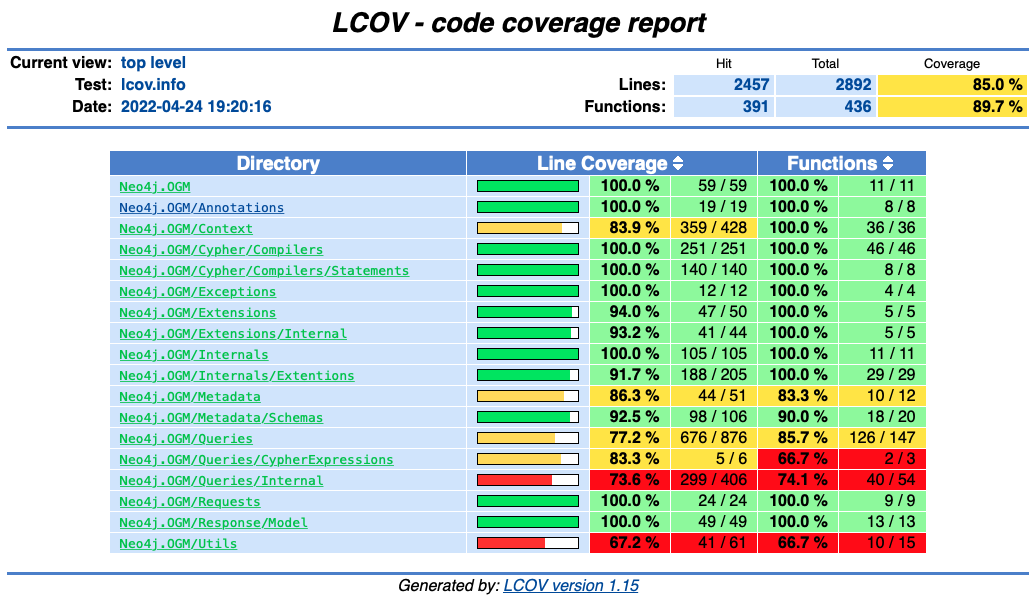
\includegraphics[width=\textwidth]{content/coverage_report.png}
    \caption{Example of the report}
    \label{fig:report}
\end{figure}
\todo[inline]{Better coverage report image}

\section{\texttt{SessionFactory} tests}

We will start with testing \texttt{SessionFactory} as it is the entry point to use our library, tests will be simple,
we want to test, that \texttt{SessionFactory.Create} return an instance of \texttt{ISession} and that if the configuration
set on creating \texttt{SessionFactory} is invalid, that proper exception will be thrown.

\subsection{Mocking}

When writing tests for \texttt{SessionFactory} we encountered a problem with sending assemblies containing our domain model to the \texttt{SessionFactory}
constructor. We want these assemblies to be mocked.

What is mocking? "Mocking is a process used in unit testing when the unit being tested has external dependencies.
The purpose of mocking is to isolate and focus on the code being tested and not on the behavior or state of external dependencies.
In mocking, the dependencies are replaced by closely controlled replacements
objects that simulate the behavior of the real ones." \cite{noauthor_mocking_nodate}

For our case, we will use a library for .NET called Moq, which is available as NuGet package, more information about this package can
be found at \url{https://github.com/moq/moq4}.

With sample \ref{code:SessionFactoryCreateTest} of one of the tests for \texttt{SessionFactory.Create}, we can see how we are applying mocking in this test.
In the code sample \ref{code:SessionFactoryCreateTest}, we are firstly creating a mock of \texttt{Assembly} class and then we also are creating a fake result for
on of the methods in the \texttt{Assembly} class. This method is used internaly inside library and we need to define our own result to be able to inject right
array of classes against we want to run test.

\begin{listing}[H]
    \begin{minted}[
 frame=lines,
 framesep=2mm,
 baselinestretch=1,
 bgcolor=LightGray,
 linenos,
 breaklines
 ] {csharp}
 public void CreateTestResultOk()
 {
     var assembly = new Moq.Mock<Assembly>();
     assembly.Setup(a => a.GetTypes()).Returns(new[] { typeof(Person), typeof(Post) });

     var sessionFactory = new SessionFactory(
        "connectionString",
        AuthTokens.Basic("username", "password"),
        assembly.Object);

     var session = sessionFactory.Create();

     Assert.NotNull(session);
     Assert.IsAssignableFrom<ISession>(session);
 }
    \end{minted}
    \caption{Example of \texttt{SessionFactory} test with mocking of \texttt{Assembly} object}
    \label{code:SessionFactoryCreateTest}
\end{listing}

\section{Testing internal classes and methods}

In our library, we are using a keyword \texttt{internal} which hides classes, methods or properties from other assemblies,
but because we want to also test these classes and their methods, we need to expose them. Exposing \texttt{internal} is possible
with small change in project file. We just need to add this \ref{code:csprojinternal} to library project file and our tests will be able to access every internal
class and method.

\begin{listing}[H]
    \begin{minted}[
 frame=lines,
 framesep=2mm,
 baselinestretch=1,
 bgcolor=LightGray,
 linenos,
 breaklines
 ] {xml}
<ItemGroup>
 <AssemblyAttribute
 Include="System.Runtime.CompilerServices.InternalsVisibleTo">
   <_Parameter1>Neo4j.OGM.Tests</_Parameter1>
 </AssemblyAttribute>
</ItemGroup>
    \end{minted}
    \caption{Edit of \texttt{Neo4j.OGM.csproj} to access internal classes and methods inside test project}
    \label{code:csprojinternal}
\end{listing}

Using this alteration of the \texttt{Neo4j.OGM.csproj} to access internal classes and methods inside test project,
we can now prepare test for internal classes and methods.

\section {Setup and cleanup}

Some of our tests will need to prepare data and mocks, we call this step of tests a setup step. nUnit for example, uses annotations
to mark cleanup (\texttt{TearDownAttribute}) and setup (\texttt{SetUpAttribute}) methods. However, in xUnit, we are using only constructors and \texttt{IDisposable}
interface for setup and cleanup respectively. This approach has a limitations in not beign able to safely perform asynchronous operations,
but xUnit has a solution for this too, \texttt{IAsyncLifetime} is an interface from xUnit, that provides means to asynchronously perform setup and cleanup
methods.

\todo[inline]{Add code example for xUnit setup and cleanup}

Appart from setup and cleanup methods, xUnit also offers an ability to share context between test, either in one class or across multiple classes
using class fixtures or collection fixtures, more on this subject can be found in official documentation of xUnit framework.



\todo[inline]{TBD}